\chapter{Mass Action Kinetics} \label{ch:mak}

One way to describe what is going on inside a cell is to suppose that
the cell is just a very small, well-mixed test tube containing all of
the molecules (proteins, RNAs, DNAs, lipids, sugars, etc.) in a
solution of $H_2O$. That is, we ignore the unseemly reality that most
of these molecules are stuck to each other, to membranes, inside
organelles, etc. If the cell really were a test tube, then the
reactions between molecules would follow the laws of {\em mass action
  kinetics}, which we describe here. Essentially: molecules react with
each other to form new molecules at rates proportional the
concentration of the reactants.

Of course, the test tube idea is not even a remotely good assumption
about what is really happening, but it does provide us with a starting
point for modeling, and often the models obtained using mass action
kinetics are fairly informative.

Chemical kinetics is a well-estabilished area in chemistry,
mathematical modeling and non-linear systems. There are several good
sources for this material, such as the notes by Martin Feinberg
\cite{feinberg-book} from which the notes here draw heavily. Here,
however, we present the mass action kinetics using a notation
consistent with the other ideas in this book, and give examples that
are related to molecular biology rather than chemistry.

\section{Definitions}

\subsection{Reaction Networks}

In general, we name the molecular {\em species} in a system $X_1$,
$X_2$, ..., $X_N$. These might be the names of particular proteins,
messenger RNAs or small molecules. In particular examples, the species
are named with capital letters like $B$, $M$ and $E$ instead of the
generic $X_i$. A {\em reaction} among the molecular species in
question has the form
%
$$
\underbrace{n_1 X_1 + ... + n_N X_N}_\mathrm{reactants}
  \rightharpoonup \underbrace{m_1 X_1 + ... + m_N X_N}_\mathrm{products} 
$$
%
where $n_1, ..., n_N, m_1,...,m_N \in \nats \cup \{0\}$. In this
reaction, $n_i$ molecules of species $X_i$ are {\em consumed} and
$m_i$ molecules of species $X_i$ are produced. A reaction can be
written more conveniently as a vector
%
\begin{equation}\label{eqn:reaction}
a = -\vvvec{n_1}{\vdots}{n_N} + \vvvec{m_1}{\vdots}{m_N} = -a_R + a_P \in \ints^N, 
\end{equation}
%
where $a_R$ is the vector of reactant numbers and $a_P$ is the vector
of product numbers. The vector $a$ is called the {\em stoichiometry} of the reaction.

\begin{example} \label{ex:reaction} Suppose we have three species $X$, $Y$ and $Z$. The single reaction 
%
$$
X + Y \rightharpoonup Z
$$
%
can be written as a vector
%
$$
a = \vvvec{-1}{-1}{1}, 
$$
%
as long as we remember that the species are always ordered as we
presented them above. \enx
\end{example}

A system inside the cell, consisting of a number of species and the
reactions among them is modeled a {\em reaction network}, which is
simply a set of reactions. The nodes of the network are {\em
  complexes} (e.g. $X+Y$ and $Z$ in the previous example) and the
edges are the reaction arrows. Furthermore, the reaction vectors
associated with the reactions in a network can be grouped into a
matrix $A$ called the {\em stiochiometric matrix}.

\begin{example} \label{ex:network}
The reactions 
\begin{eqnarray}
X + Y & \rightharpoonup & Z \\
2Z & \rightharpoonup & X
\end{eqnarray}
%
form a reaction network with stiochiometric matrix
%
$$
A = \left ( \begin{array}{cc}
-1 & 1 \\
-1 & 0 \\
1 & -2
\end{array} \right ).
$$
%
\enx
\end{example}

\subsection{Kinetics}

In a system of reacting chemicals, the state at a particular time is
described by the {\em concentrations} of each species, usually
arranged into another vector. If $X_i$ is a species, then we write
$v_{X_i}(t)$ or just $v_i(t)$ to represent the number of molecules of
species $X_i$ per unit volume at time $t$. Then we group the
concentrations into a vector
%
$$
v = \vvvec{v_1}{\vdots}{v_n} \in \positives^N.
$$
%
It is generally assumed that the number of molecules in the
system is very large, so that stochastic effects do not come into
play. For this reason, we may call the model described in this chapter
as the {\em deterministic} model to contrast it with the {\em
  stochastic} model to be described in Chapter \ref{ch:cme}.

Associated with each reaction $a$ is a {\em reaction rate} 
%
$$
K_a : \positives^N \rightarrow \positives
$$
%
that depends on the concentrations. If $K_a(v) > 0$ then every
reactant in $a$ has nonzero concentration in the state $v$. Reaction
rates, when noted, are usually written above the reaction arrows in a
specification of the reaction. A {\em kinetics} for a network is such
an assignment of a rate to each reaction $a$. These rates may be
grouped into a vector $K(v)$ that depends on $v$:
%
$$
K(v) = \vvvec{K_{a_1}(v)}{\vdots}{K_{a_M}(v)}, 
$$
%
where we have numbered the reactions from $1$ to $M$.

The usual assumption is that the kinetics obey the {\bf law of mass
  action}, although they need not. In later chapters we will allow
the rates to be defined in other ways. For now, however, we stick with
the following definition of the rates. 

\begin{definition}
  Suppose that $a$ is defined as in \eref{eqn:reaction}. Then the
  {\em mass action rate} for the reaction $a$ os definted by
%
\begin{equation}\label{eqn:mak-rate}
K_a(v) \defeq k_a \prod_{i}v_i^{n_i}
\end{equation}
%
where $k_a$ is called the {\em rate constant} for the reaction
$a$. 
\end{definition}

The idea the following. Suppose that an $X$ molecule reacts with
a $Y$ molecule according to the reacton
%
$$
X + Y \xrightharpoon[\text{}]{\text{$k$}} Z
$$
%
If there are $v_X$ molecules of type $X$ per liter and $v_Y$ molecules
of type $Y$ per liter, then the number of possible reactions that can
occur per liter is $v_X v_Y$. Since some types of reactions may be
stronger or faster than others, we add a rate constaint $k$ to our
model to obtain $kv_Xv_Y$. When the rate constant is important, we
make a note of it by writing it, as above, near the arrow used to
specify the reaction.  The definition \eref{eqn:mak-rate} is a
generalization of the idea of having the rate of a reaction include a
term that desribes the number of ways that a reaction can happen: the
rate is proporional to the current concentrations, or masses, of the
reactants.

\begin{example} \label{ex:mak}
The reaction rates for the reactions in Example~\ref{ex:network} are
$$
K(v) = \vvec{k_1 v_X v_Y}{k_2 v_Z^2}
$$
%
where we suppose that $k_1$ and $k_2$ are the rate constants for the two reactions in
the network respectively. \enx
\end{example}

\subsection{The Determinstic Equations}

The rate at which the concentrations in a reaction network change
leads to a set of differential equations, called the deterministic
equations (to contrast them with the stochastic equations we study
later) that can be written succinctly as
%
\begin{equation} \label{eqn:mak}
\dot v = A K(v) .
\end{equation}
%
Along with an initial concentration vector $v(0)$ and actual values
for the rate constants, this completely specifes the behavior of a
reaction network.

\begin{example} Applying  \eref{eqn:mak} to the stoichiometric matrix $A$ in
  Example~\ref{ex:network} and the rate vector $K(v)$ in
  Example~\ref{ex:mak} gives
%
$$
\vvvec{\dot v_X}{\dot v_Y}{\dot v_Z} = A K(v) 
  = \vvvec{-k_1 v_X v_Y + k_2 v_Z^2}{-k_1 v_X v_Y}{k_1 v_X v_Y - 2 k_2 v_Z} ,
$$
%
which is simply a list of three equations stating how the
concentrations of $X$, $Y$ and $Z$ in the network change over time. \enx
\end{example}

\subsection{Basic Properties}

The mass action kinetics equations for a given network are, in
general, nonlinear. Explicit, closed-form solutions for the equations
do not exist except in simple situations. However, systems of
differential equations arising from mass action kinetics are not
entirely arbitrary either, and all mass action systems obey some
simple properties, which we now discuss.

The first property states that concentrations can never be negative as
long as they start out positive. This property is certianly true of
actual physical systems. Mathematically, the property holds because if
a concentration ever becomes zero, its rate of change is necessarily
non-negative.

\begin{property} \label{prop:nonneg} If $v \in \positives$ and
  $v_i=0$, then $\dot v_i \geq 0$.
\end{property}

\begin{proof}
  Every reaction $a$ in which $X_i$ shows up as a reactant has $K_a(v)=0$
  whenever $K_a(v)$ is defined by Equation~\eref{eqn:mak}. Thus 
  contributions to $\dot v_i$ are only from reactions in which $X_i$
  appears as a {\em product} and are therefore non-negative. 
\end{proof}

The next property describes the set of all possible concentration
vectors that can be reached starting from a given initial
condition. We first require a definition:

\begin{definition}\label{def:stoich-sub}
The {\em stoichiometric subspace} of a system with matrix $A = (a_1,...,a_N)$ is
%
\begin{eqnarray*}
S & = & \mathrm{span} A = \mathrm{span} \{ a_1, ..., a_N \} \\
  & = & \{ r_1 a_1 + ... + r_N a_N \;|\; r_1, ..., r_N \in \reals \}. 
\end{eqnarray*}
The {\em rank} of a reaction network is the rank of $S$ (i.e. the
number of linearly independent columns or rows). If $v_1-v_2 \in S$,
then $v_1$ and $v_2$ are said to be {\em stoichiometrically
  equivalent}.
%
\end{definition}

\begin{example} \label{ex:span}
Suppose that
$$
A = \left ( \begin{array}{cc}
-1 & 1 \\
-1 & 0 \\
1 & -2
\end{array} \right ).
$$
as in Example~\ref{ex:network}. Then
%
$$
S = \left \{ \vvvec{r_2-r_1}{-r_1}{r_1-2r_2} \;|\; r_1,r_2 \in \reals \right \}. 
$$
%
In this case, $S$ is a two dimensional subspace of $\reals^3$, suggesting
that the three differential equations we use to describe it are
redundant in some way. \enx
\end{example}

The notion of {\em stiochiometrically equivalent} leads to equivalence
classes of states and the simple property that all solutions of a mass
acton kinetics system remain in an equivalence class defined by the
initial condition. This is characterized in the following property.

\begin{property} \label{prop:equiv}
All solutions $v(t)$ of 
%
$$
\dot v = A K(v) \;\;\;\;\; \mathrm{with} \; v(0) \; \mathrm{given}
$$
%
lie in the stochiometric equivalence class of $v(0)$. I.e. $v(t)$ is
always stoichiometrically equivalent to $v(0)$. 
\end{property}

\begin{proof} The property follows from the definition of the
  derivative and of $S$:
$$\dot v = \lim_{h \rightarrow 0} \frac{v(t+h)-v(t)}{h} = A K(v) \in S.$$
\end{proof}

These notions can be best seen in a two-dimensional example.

\begin{example} \label{ex:stoich}
Consider the network
%
$$
X \xrightleftharpoons[\text{$k_2$}]{\text{$k_1$}} 2 Y 
$$
%
with the initial condition defined by $v_X(0)=1$ an $v_Y(0)=0$. The
stiochiometric matrix is
%
$$
A = \left ( \begin{array}{cc}
-1 & 1 \\
2 & -2
\end{array} \right )
$$
%
and
%%
$$
S = \left \{ \vvec{-r}{2r} \;|\; r \in \reals \right \}. 
$$
%%
By Property \ref{prop:equiv}, for every $t$ there exists an $r$ such that
%
$$
v(t) - v(0) = \vvec{v_X(t)}{v_Y(t)} - \vvec{1}{0} = \vvec{-r}{2r}
$$
%
from which it follows that all $v(t)$ have form
%
$$
\vvec{1-r}{2r} .
$$
%
Furthermore, since all concentrations must be non-negative, $r \in
[0,1]$. We can further analyze this system be looking at the locus of
equilibra. Setting
%%
$$
\dot v = A K(v) = \vvec{-k_1 v_X + k_2 v_Y^2}{k_1 v_X - k_2 v_Y^2} = 0,
$$
%%
we get $k_1 v_X = k_2 v_Y^2$ or $v_X = \frac{k_2}{k_1} v_Y^2$. The
general picture is shown in Figure~\ref{fig:stoich}. 
\end{example}

\begin{example}
  Continuing with the previous example, we note that the system is
  really one dimensional. We can write it in terms of $r$ in fact as
  follows:
%
\begin{eqnarray*}
\dot r & = & \frac{\dot v_Y}{2} \\
       & = & \frac{1}{2} \left ( k_1 v_X - k_2 v_Y^2 \right ) \\
       & = & \frac{1}{2} \left ( k_1 (1-r) - k_2 (2r)^2 \right ) \\
       & = & \frac{k_1}{2}(1-r) - 4 k_2 r^2 .
\end{eqnarray*}
%
Anything true abut this equation can be translated back to statements
about the original set of equations. \enx
\end{example}

\begin{figure}

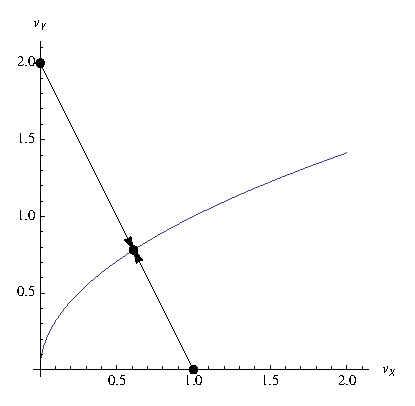
\epsfig{file=figures/stoich-sub.eps}

  \caption{\label{fig:stoich} The stoichiometric subspace from
    Example~\ref{ex:stoich} is a one-dimensional line connecting
    $(1,0)$ to $(0,2)$. The points on this line tend toward the point
    where stoichiometric subspace intersects the locus of equilibra}

\end{figure}

\section{Example Networks}

\subsection{Sources and Sinks}

If $a_r = 0$, then the species in $a_p$ appear from nowhere. Thus,
$a_r=0$ models a {\em source}. We write, equivalently,
%
$$
0 \rightharpoonup a_p
$$
%
and 
%
$$
\varnothing \rightharpoonup m_1 X_1 + ... + m_N X_N .
$$
%
Similarly, if $a_p = 0$, then reactants can disappear from the system
and $a_p=0$ is called a {\em sink}. 

\begin{example}
The reaction 
%
$$
\varnothing \xrightharpoon[\text{}]{\text{$k$}} A
$$
%
has the mass action kinetics
%
$$
\dot v_A = k.
$$
%
That is, $A$ is added to the system at a constant rate.
\enx
\end{example}

\begin{example}
The reaction 
%
$$
A \xrightharpoon[\text{}]{\text{$k$}} \varnothing 
$$
%
has the mass action kinetics
%
$$
\dot v_A = - k v_A.
$$
%
That is, the more $A$ is in the system, the faster its concentration
decreases. \enx
\end{example}

\subsection{Constant Concentrations}

In the cell, many species are regulated using feedback so that they
maintain essentially constant levels. For example, ATP -- the basic
unit of energy -- is regulated tightly \cite{ATP_IS_REGULATED}. ATP is
also involved in many reactions. We could include ATP as a reactant or
product in all of the reactions in our network, but because it is
regulated, we would also have to include the regulation machinery in
our model as well. To get around this, we usually just pretend that
$\dot v_{ATP}=0$ and write, for example,
%
$$
X  \xrightharpoon[\text{}]{\text{$k v_{ATP}$}} Y
$$
%
to denote that the rate at which $X$ is converted into $Y$ depends on
the concentration of $ATP$. The above reaction gives the kinetics
%
$$
\dot v_X = - \dot v_Y = - k v_{ATP} v_X 
$$
%
where $v_{ATP}$ does not depend on time (i.e. it is a constant
parameter in our model). 

\subsection{Membranes}

Say $X$ and $Y$ react according to the reaction
%
$$
X  \xrightleftharpoons[\text{$k_2$}]{\text{$k_1$}} 2 Y 
$$
%
in two compartments separated by a membrane with some active transport
mechanism across it, as in Figure~\ref{fig:membrane}. To model this
system with mass action kinetics, we define new symbols $X_1$ and
$X_2$ to refer to $X$ molecules when they are in compartent one and
compartment two, respectively. Similarly, we introduce the names $Y_1$
and $Y_2$. We can the write the reaction network

\begin{center}
\begin{tabular}{ccc}
$X_1  \xrightleftharpoons[\text{$k_2$}]{\text{$k_1$}} 2 Y_1$ & \ \ \ \ \ & $X_1  \xrightleftharpoons[\text{$k_4$}]{\text{$k_3$}} X_2$ \\
\ & \ & \\
$X_2  \xrightleftharpoons[\text{$k_2$}]{\text{$k_1$}} 2 Y_2$ & \ \ \ \ \ & $Y_1  \xrightleftharpoons[\text{$k_6$}]{\text{$k_5$}} Y_2$ 
\end{tabular}
\end{center}

\noindent
which describes a system with four ``species'' that model our two
species reacting in a two-compartment system.

\subsection{Conservative Systems}

For the system 
%
$$
X  \xrightleftharpoons[\text{$k_2$}]{\text{$k_1$}} 2 Y 
$$
%
we can define a vector $m$ by
%
$$
m = \vvec{2}{1}
$$
%
and note that
%%
\begin{eqnarray*}
\frac{d}{dt} m^T v & = & m^T \dot v = m^T A K(v) \\
 & = & (2 \; 1) {\left ( \begin{array}{cc} 
  -1 & 1 \\
  2  & -1 \end{array} \right ) K(v) } \\
 &   & \\
 & = & ( 0 \; 0 ) K(v) = 0 .
\end{eqnarray*}
%%
The idea is that $X$ molecules have twice the mass of $Y$ molecules
and $m$ records this fact. The quantity $m^Tv$ is the total mass of
the system over all species. Its derivative is zero because mass in
conserved in this system. 

In contrast, the system
%
$$
X  \xrightharpoon[\text{}]{\text{$k_1$}} 2 Y 
$$
%
$$
Y  \xrightharpoon[\text{}]{\text{$k_2$}} X
$$
%
where $Y$ decays back into a single $X$ (forgetting that it seems to
have been constructed out of two $X$ molecules) does not have a
meaningful mass vector. This is because
%
$$
m^T A = ( m_X \; m_Y ) \left ( \begin{array}{cc} 
  -1 & 1 \\
  2  & -1 \end{array} \right ) = \vvec{0}{0}
$$
%
has no non-trivial solution. In this case, the network is not conservative. 

Another possibility is that $m^TA=0$ may have no positive solution. A
negative solution would lead to a strange definition of mass. These
ideas motivate the following definition. First, recall that if we are
given a subspace $S$ of a vector space $V$, the {\em orthogonal
  compliment} of $S$ is 
%
$$
S^\bot = \{ u \in V \;|\; u^Tv = 0, \; \forall v \in S \} . 
$$

\begin{definition} \label{def:conservative} A reaction network with
  stoichiometric subspace $S$ is conservative if there is a positive
  vector $m$ contained in $S^\bot$. 
\end{definition}

To find a mass vector, then, one has to solve $m^TA$ for $m$ and see
if $m$ can be positive. This amounts to solving a system of linear
equations, which can be done with Gaussian elimnation, for example.

\begin{figure}
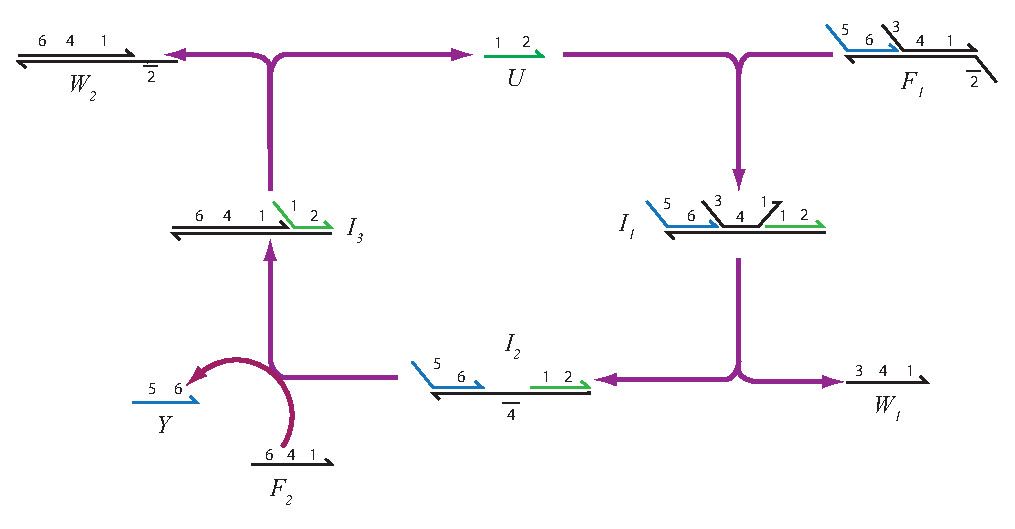
\epsfig{file=figures/zhang-integrator.eps, scale=0.75}
\caption{\label{fig:zhang-integrator} A DNA hybridization circuit from
  \cite{zhang-integrator}. Each line represents a single stranded
  piece of DNA. Parallel lines correspond to double stranded
  DNA. Numbers denote binding domains, which are unique seqnences of
  A, T, C or G nucleotides. A number with a bar denotes a
  complimentary sequence.}
\end{figure}

\begin{example}\label{ex:zhang-integrator}
  Consider the network in Figure~\ref{fig:zhang-integrator}. In it,
  oligonucleotides form and unform complexes of one or more
  oligos. Thus each complex is a species, but it is also made up of
  individual oligos, suggesting that the number of oligos in a complex
  should be the mass of the complex. For this system, we have the
  following reactions (ignoring the rates for now).
%
\begin{eqnarray*}
U + F_1 & \rightharpoonup & I_1 \\
I_1 & \rightharpoonup & W_1 + I_2 \\
I_2 + F_2 & \rightharpoonup & I_3 + Y \\
I_3 & \rightharpoonup & W_2 + U .
\end{eqnarray*}
%
If we define $v = ( U \; F_1 \; F_2 \; I_1 \; I_2 \; I_3 \; W_1 \; W_2 \; Y )^T$
then a suitable mass vector is
%
$$
m = ( 1 \; 3 \; 1 \; 4 \; 3 \; 3 \; 1 \; 2 \; 1 ) ,
$$
%
where the mass of each species is given by the number of oligos in
it. This fact is confirmed in an exercise.  \enx
\end{example}

\section{Modeling Regulatory Networks and Metabolism}

% Put a bunch of snippets of GRNs and 
%
% start with a single gene
% then a gene with a repressor
% then one with an activator
% then one with some protein-protein intreaction, like in the ARF system
%

% A <-> B -> C : Show that increasing forward and reverse rate of first 
% reaction 

In this section we explore how mass action kinetics can be used to
model genetic regulatory networks and metabolism. We start by modeling
a single gene, and then simple combinations of genes. Finally, we show
an example from metabolism. In the next chapter we show how the
systems here can be simplified to some extent using a set of
approximation called {\em enzyme kinetics}. 

\begin{example} \label{ex:onegene}
  Consider a single consitutively expressed gene producing a single
  protein $X$ at a rate $k_1$. The protein is degraded and diluted due
  to cell growth at a rate $k_2$. Note that the concentration of RNAP,
  like ATP above, is regulated and, therefore, does not appear in
  these reactions. Instead it is absorbed into the rate constant
  $k_1$. Similarly, the concentration of proteins that degrade protein
  is absorbed into $k_2$. A simple model of our system is then
%
$$
\varnothing \xrightharpoon[\text{}]{\text{$k_1$}} X \xrightharpoon[\text{}]{\text{$k_2$}} \varnothing
$$
%
which gives the differential equation
%
$$
\dot v_X = k_1 - k_2 v_X.
$$
%
A more sophisticated model of this system includes the messenger RNA
intermediate. Let's call it $R$. The gene produces $R$ and $R$
produces proteins before being degraded and
diluted. Adding these complexities to our model gives
%
$$
\varnothing \xrightharpoon[\text{}]{\text{$\kappa_1$}} R \xrightharpoon[\text{}]{\text{$\kappa_2$}} \varnothing
$$
%
%
$$
R \xrightharpoon[\text{}]{\text{$\kappa_3$}} R + P 
$$
%
%
$$
P \xrightharpoon[\text{}]{\text{$\kappa_4$}} \varnothing
$$
%
The second line, where $R$ produces $P$ shows that the mRNA is not
consumed in the process of being transcribed into protein. Note also
that the concentration of ribosomes is absorbed into $\kappa_3$. 
The above system gives rise to the equations
%
\begin{eqnarray*}
\dot v_R & = & \kappa_1 - \kappa_2 v_R \\
\dot v_P & = & \kappa_3 v_R - \kappa_4 v_P .
\end{eqnarray*}
%
One might ask: {\em What values of $k_i$ and $\kappa_i$ make these two
  descriptions similar?} To answer this, note that the rate of
production and degradation of mRNA is faster than with protein. Thus,
we can assume that the level of mRNA equilibrates quickly, meaning that
%
$$
\dot v_R = \kappa_1 - \kappa_2 v_R = 0
$$
%
which implies that $R = \kappa_1/\kappa_2$ fairly soon. Thus, the
equation for protein production becomes
%
$$
\dot v_P = \kappa_3 \frac{\kappa_1}{\kappa_2} v_R - \kappa_4 v_P .
$$
This implies that 
%
$$
k_1 = \frac{\kappa_3\kappa_1}{\kappa_2} \;\;\;\mathrm{and} \;\;\; k_2 = \kappa_4 . 
$$
%
A simulation of these two systems is shown if
Figure~\ref{fig:onegene}. Note that the main difference in the two
curves is that initially, $\dot v_P = 0$ in the more complex
model. This may be an insignificant difference in some situations, but
in others in is crucially important (as in Example~\ref{ex:repressilator}). 
\enx
\end{example}

\begin{figure}
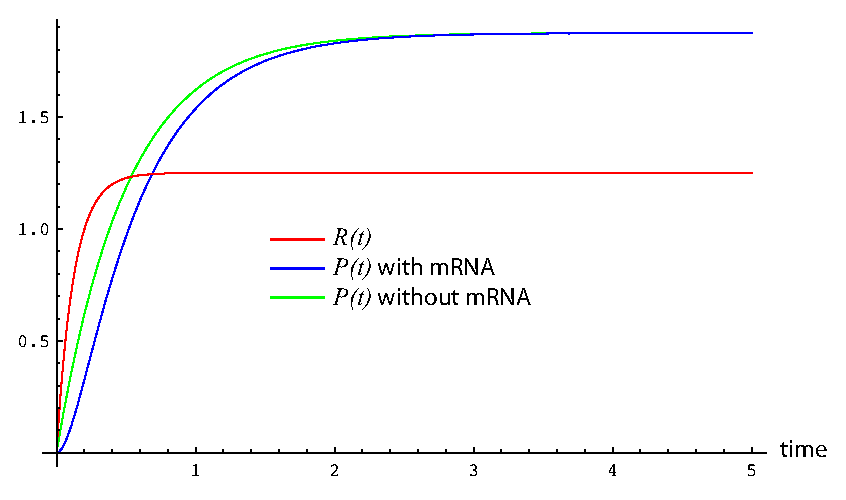
\epsfig{file=figures/one_gene.eps, scale=0.7}
\caption{\label{fig:onegene}
Two models of gene expression, one modeling mRNA explicitly and the other not. 
}
\end{figure}

\begin{example} \label{ex:repression}
  Now consider a gene $g$ that produces a protein product $X$ that is
  repressed by a transcription factor $T$. In reactions, this can be written
%%
$$
g \xrightharpoon[\text{}]{\text{$k_1$}} g + P 
$$
$$
P \xrightharpoon[\text{}]{\text{$k_2$}} \varnothing
$$
$$
T + g \xrightleftharpoons[\text{\text{$k_4$}}]{\text{$k_3$}} g_\mathrm{off} .
$$
%%
The first reaction models the fact that the gene $g$ produces a
protein product $P$ at some rate, without itself being consumed. The
second reaction models protein degradation. The third line models the
interaction between the transcription factor $T$ and the gene
$g$. When $T$ is bound to $g$, RNAP is unable to bind to $g$ to
produce $P$, thus the name $g_\mathrm{off}$. Note that there is a
conservation of mass with $g$ and $g_\mathrm{off}$. Namely, there is
some constant $C$ such that
%
$$
v_g + v_{g_\mathrm{off}} = C.
$$
%

We now consider the steady state concentration of $P$ for varying
input concentrations of $T$. Since
$$
\dot v_P = k_1 v_g - k_2 v_P, 
$$
we have $v_P^* = k_1 v_g^* / k_2$. The dynamics of $g$ are given by
$$
\dot v_g = -k_3 v_T v_g + k_4 ( C - v_g ) 
$$
so that
$$
v_g^* = \frac{k_4  C}{k_3 v_T + k_4} . 
$$
Thus, by substituting the above into the equation for the steady state
concentration of $P$, we can see it is inversely related to the
concentration of $T$:
$$
v_P^* = \frac{k_1 k_4  C}{k_2 k_3 v_T + k_2 k_4} . 
$$
In the next chapter we study these kinds of relationships more extensively.
\enx
\end{example}

\begin{example} \label{ex:repressilator}
The repressilator.
\end{example}

\begin{example}
Relaxation oscillator.
\end{example}



\section{Problems}

\setcounter{exercount}{0}

\begin{exercise} Find the stable equilibrium in Example~\ref{ex:span}
  assuming $k_1=k_2=1$.\end{exercise}

\begin{exercise} The system in Example~\ref{ex:network} is really
  two-dimensional. Write the equations in terms of $\dot r_1$ and
  $\dot r_2$ to show this.\end{exercise}

\begin{exercise} Confirm that $m$ defined in Example~\ref{ex:zhang-integrator} is
  indeed a mass vector by writing the stiochiometric matrix for the
  system and pre-multiplying it by $m$. \end{exercise}

\begin{exercise}
Consider ther system
%%
$$
2X+Y \xrightharpoon[\text{}]{\text{$1$}} X+2Y .
$$
%%
\begin{enumerate}
\item[a)] Find the stoichiometric matrix $A$ and the kinetics vector
  $K(\vec v)$. Use these to find the mass action equations.
\item [b)] Find the stochiometric subspace and its dimension.
\item [c)] Pick a reasonable initial condition and describe its
  stoichiometric equivalence class.
\item [d)] If the system is conservative, determine a mass vector. Or
  state why the system is not conservative.
\item [e)] Determine the equilibrium points of the network, the
  Jacobians evaluated at these points, and the stability of the
  points.
\item [f)] Draw a vector flow field for the network.
\end{enumerate}
\end{exercise}

\begin{exercise}
Repeat the steps in  for the following network
\begin{eqnarray*}
X & \xrightharpoon[\text{}]{\text{$1$}} & 2X \\
X+Y & \xrightharpoon[\text{}]{\text{$1$}} & 2Y \\ 
Y & \xrightharpoon[\text{}]{\text{$2$}} & \varnothing .
\end{eqnarray*}
\end{exercise}

\begin{exercise}
  Show that the two models of protein production from a single gene in
  Example~\ref{ex:onegene} give the same steady state amount of
  protein.
\end{exercise}

\begin{exercise}
Consider the system
%%
$$
\varnothing \xrightleftharpoons[\text{\text{$1$}}]{\text{$1$}} X  \xrightharpoon[\text{}]{\text{$3$}} Y
$$
$$
2X+Y \xrightharpoon[\text{}]{\text{$1$}} 3 X .
$$
Find the equilibria and determine their local stability. What do the
imaginary parts of the eigenvalues mean? Simulate the system from a
variey of initial conditions and describe the behavior obtained.
%%
\end{exercise}
